\section{findtablewidget Class Reference}
\label{classfindtablewidget}\index{findtablewidget@{findtablewidget}}
{\tt \#include $<$findtablewidget.h$>$}

\subsection*{Public Member Functions}
\begin{CompactItemize}
\item 
{\bf findtablewidget} (QWidget $\ast$parent=0)
\item 
virtual {\bf $\sim$findtablewidget} (void)
\item 
void {\bf clear\_\-all} (void)
\item 
void {\bf add\_\-row} (QString title, QString branchname, QString tags, QString\-List path, int num\_\-in\_\-recordtable)
\item 
void {\bf update\_\-columns\_\-width} (void)
\end{CompactItemize}
\subsection*{Private Slots}
\begin{CompactItemize}
\item 
void {\bf select\_\-cell} (int row, int column)
\end{CompactItemize}
\subsection*{Private Member Functions}
\begin{CompactItemize}
\item 
void {\bf setup\_\-ui} (void)
\item 
void {\bf setup\_\-signals} (void)
\item 
void {\bf assembly} (void)
\item 
bool {\bf event\-Filter} (QObject $\ast$o, QEvent $\ast$e)
\end{CompactItemize}
\subsection*{Private Attributes}
\begin{CompactItemize}
\item 
QTable\-Widget $\ast$ {\bf findtableview}
\end{CompactItemize}


\subsection{Detailed Description}




Definition at line 10 of file findtablewidget.h.

\subsection{Constructor \& Destructor Documentation}
\index{findtablewidget@{findtablewidget}!findtablewidget@{findtablewidget}}
\index{findtablewidget@{findtablewidget}!findtablewidget@{findtablewidget}}
\subsubsection{\setlength{\rightskip}{0pt plus 5cm}findtablewidget::findtablewidget (QWidget $\ast$ {\em parent} = {\tt 0})}\label{classfindtablewidget_d653e969acddfa20ca21e34dca7b40f5}




Definition at line 12 of file findtablewidget.cpp.

References assembly(), clear\_\-all(), setup\_\-signals(), and setup\_\-ui().

Here is the call graph for this function:\begin{figure}[H]
\begin{center}
\leavevmode
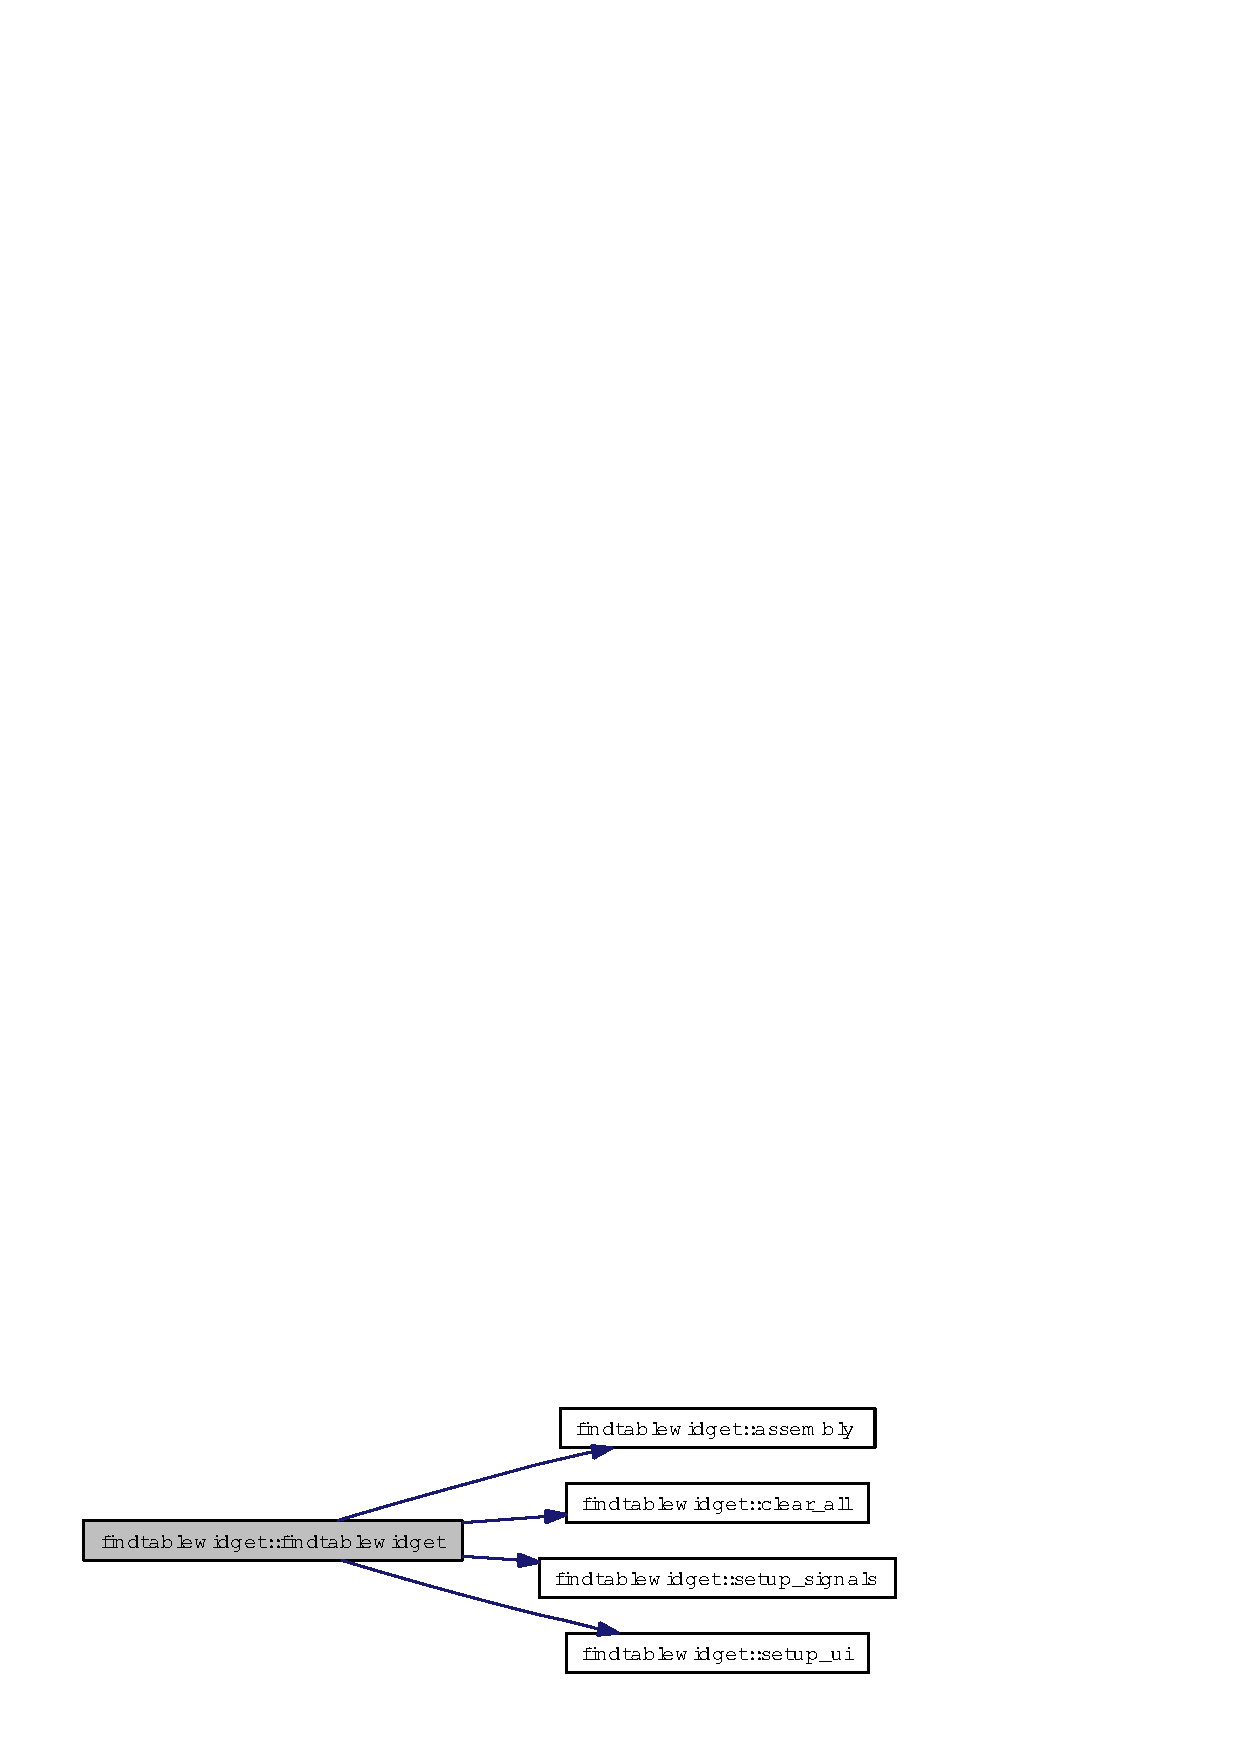
\includegraphics[width=217pt]{classfindtablewidget_d653e969acddfa20ca21e34dca7b40f5_cgraph}
\end{center}
\end{figure}
\index{findtablewidget@{findtablewidget}!~findtablewidget@{$\sim$findtablewidget}}
\index{~findtablewidget@{$\sim$findtablewidget}!findtablewidget@{findtablewidget}}
\subsubsection{\setlength{\rightskip}{0pt plus 5cm}findtablewidget::$\sim$findtablewidget (void)\hspace{0.3cm}{\tt  [virtual]}}\label{classfindtablewidget_08b5c9450513c0f36e5d20c0d401c0d0}




Definition at line 22 of file findtablewidget.cpp.

\subsection{Member Function Documentation}
\index{findtablewidget@{findtablewidget}!clear_all@{clear\_\-all}}
\index{clear_all@{clear\_\-all}!findtablewidget@{findtablewidget}}
\subsubsection{\setlength{\rightskip}{0pt plus 5cm}void findtablewidget::clear\_\-all (void)}\label{classfindtablewidget_650cffb5374085b37d54d3c59280883e}




Definition at line 73 of file findtablewidget.cpp.

References findtableview.

Referenced by findscreen::find\_\-start(), and findtablewidget().

Here is the caller graph for this function:\begin{figure}[H]
\begin{center}
\leavevmode
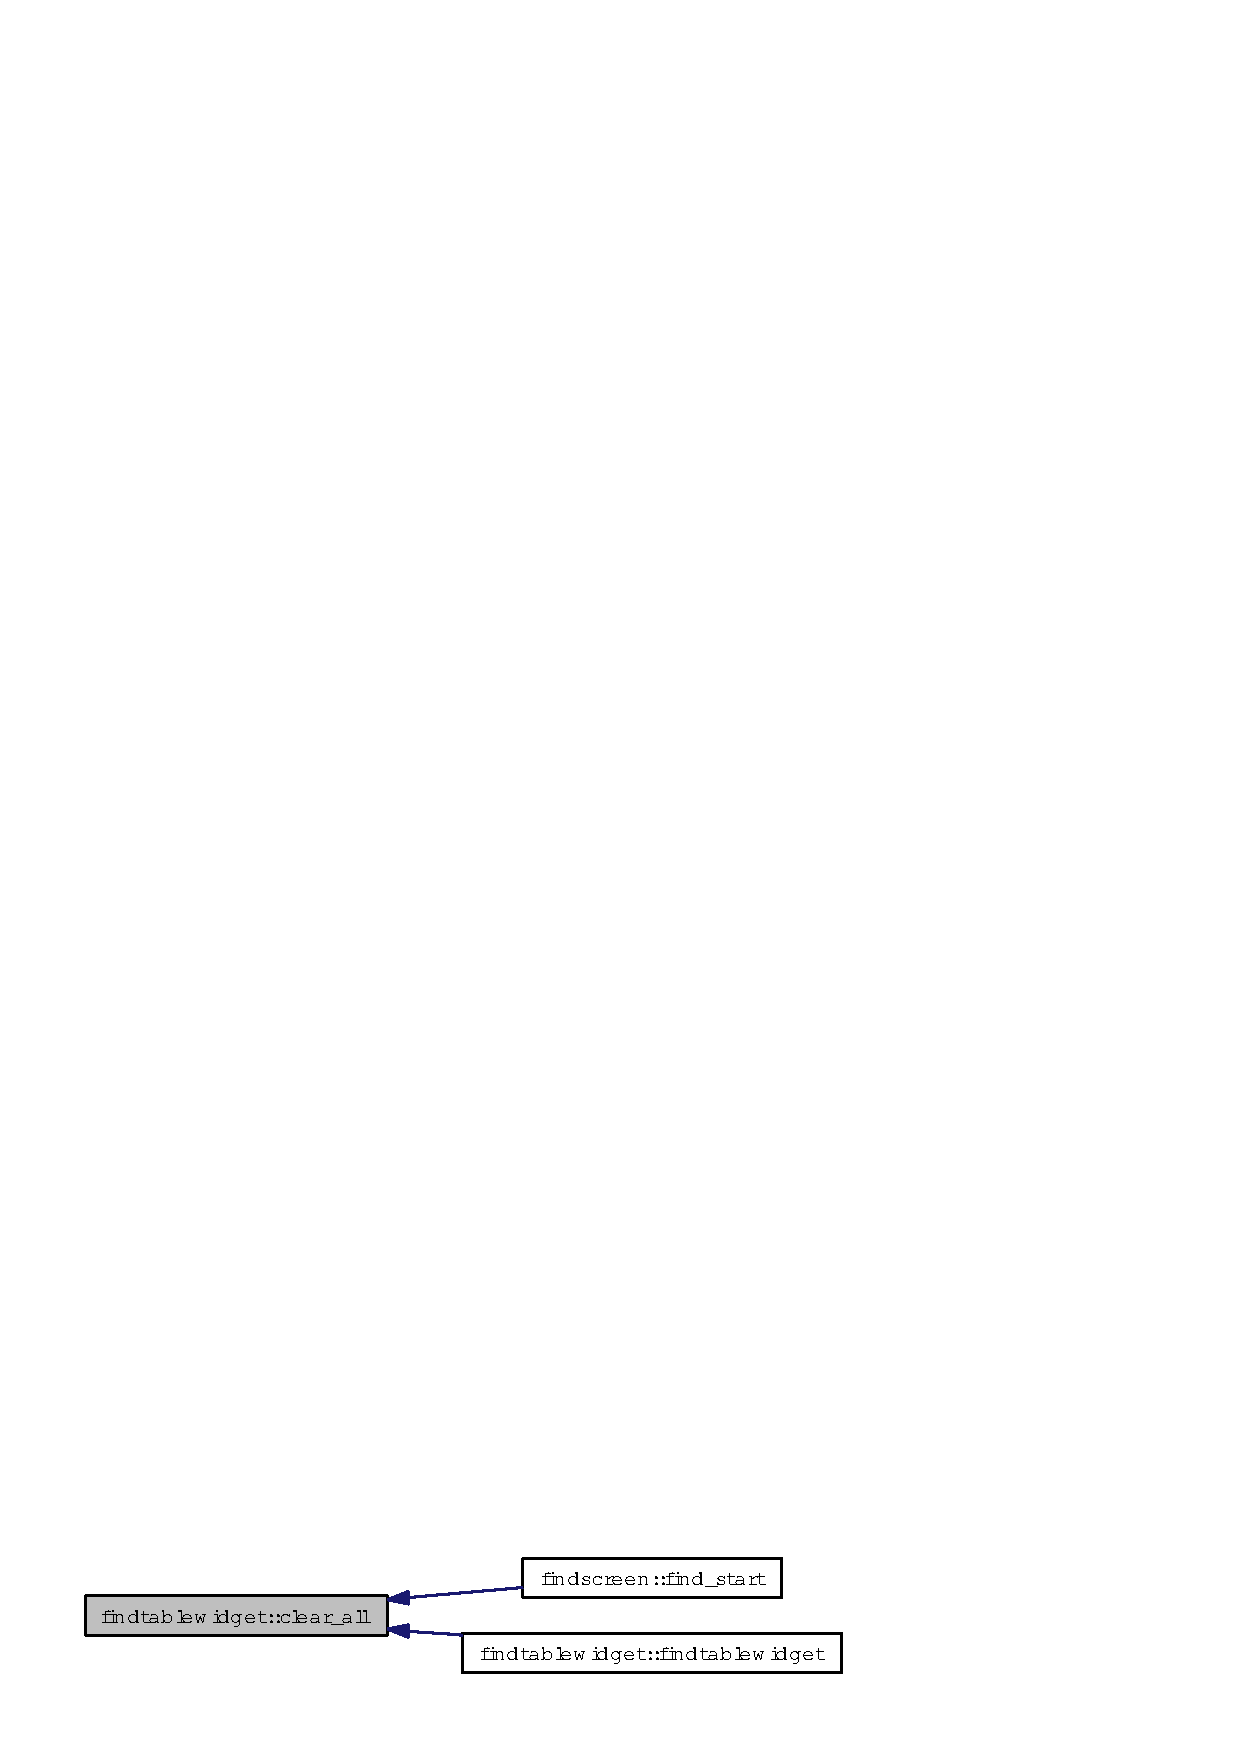
\includegraphics[width=204pt]{classfindtablewidget_650cffb5374085b37d54d3c59280883e_icgraph}
\end{center}
\end{figure}
\index{findtablewidget@{findtablewidget}!add_row@{add\_\-row}}
\index{add_row@{add\_\-row}!findtablewidget@{findtablewidget}}
\subsubsection{\setlength{\rightskip}{0pt plus 5cm}void findtablewidget::add\_\-row (QString {\em title}, QString {\em branchname}, QString {\em tags}, QString\-List {\em path}, int {\em num\_\-in\_\-recordtable})}\label{classfindtablewidget_dcb157f224ebcada52420cda81c1cb41}




Definition at line 92 of file findtablewidget.cpp.

References findtableview.

Referenced by findscreen::find\_\-recurse().

Here is the caller graph for this function:\begin{figure}[H]
\begin{center}
\leavevmode
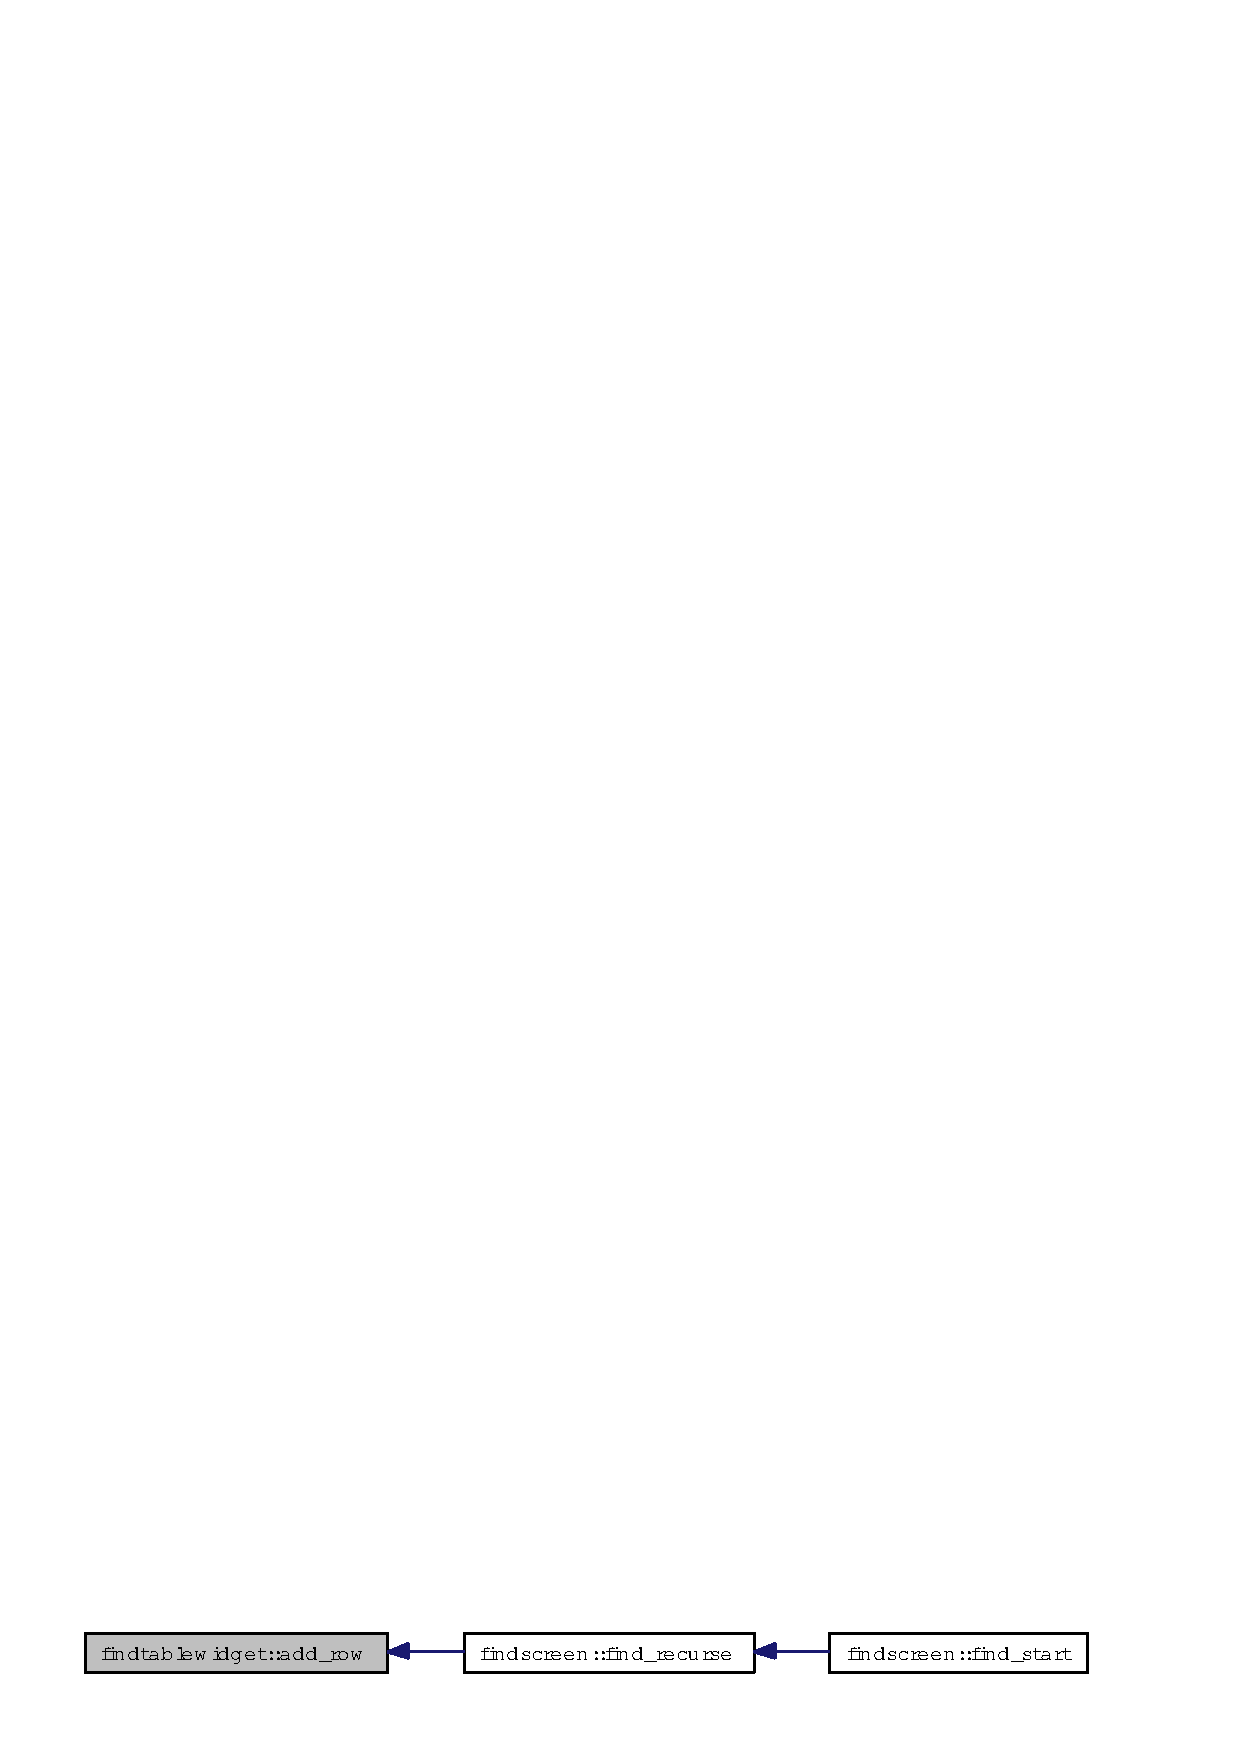
\includegraphics[width=263pt]{classfindtablewidget_dcb157f224ebcada52420cda81c1cb41_icgraph}
\end{center}
\end{figure}
\index{findtablewidget@{findtablewidget}!update_columns_width@{update\_\-columns\_\-width}}
\index{update_columns_width@{update\_\-columns\_\-width}!findtablewidget@{findtablewidget}}
\subsubsection{\setlength{\rightskip}{0pt plus 5cm}void findtablewidget::update\_\-columns\_\-width (void)}\label{classfindtablewidget_a62b6bee62382397fda46862da6f97b5}




Definition at line 65 of file findtablewidget.cpp.

References findtableview.

Referenced by findscreen::find\_\-start().

Here is the caller graph for this function:\begin{figure}[H]
\begin{center}
\leavevmode
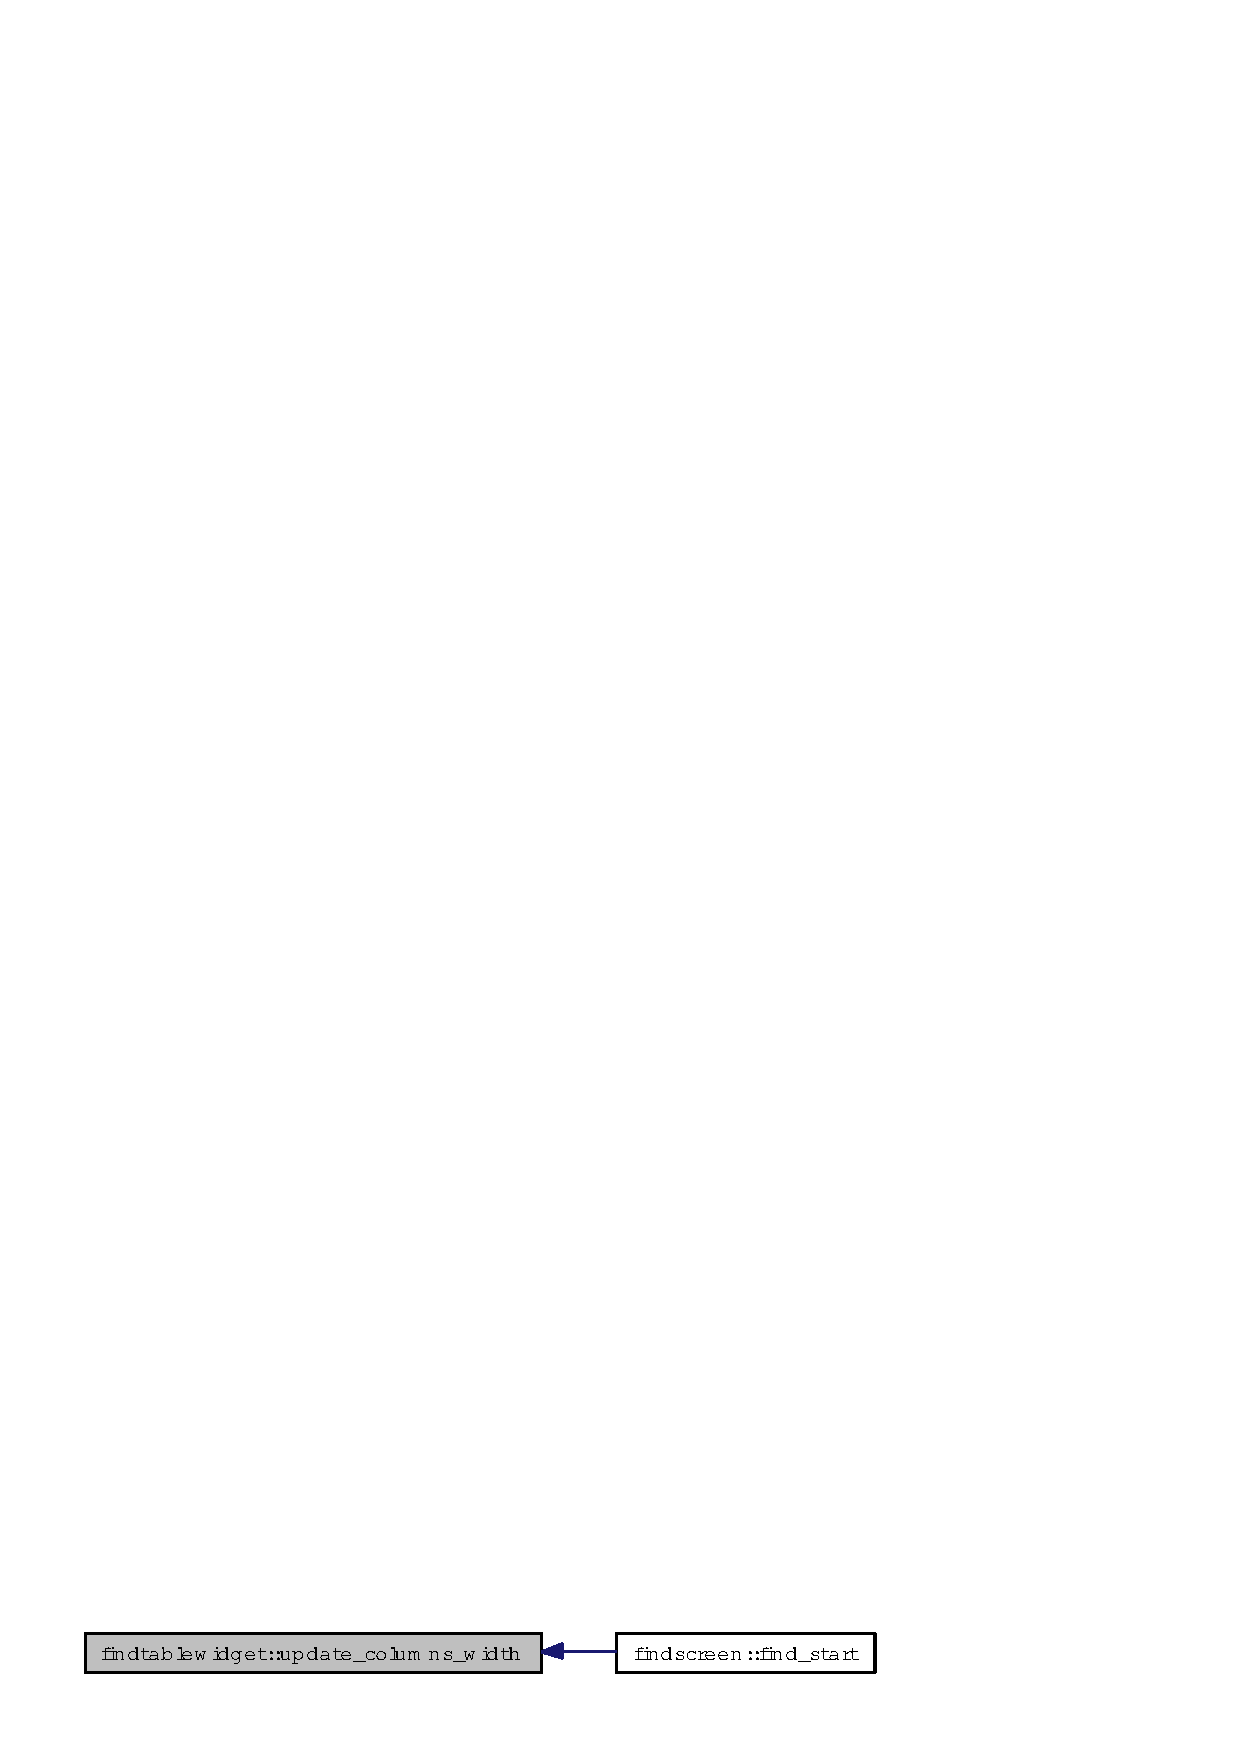
\includegraphics[width=212pt]{classfindtablewidget_a62b6bee62382397fda46862da6f97b5_icgraph}
\end{center}
\end{figure}
\index{findtablewidget@{findtablewidget}!select_cell@{select\_\-cell}}
\index{select_cell@{select\_\-cell}!findtablewidget@{findtablewidget}}
\subsubsection{\setlength{\rightskip}{0pt plus 5cm}void findtablewidget::select\_\-cell (int {\em row}, int {\em column})\hspace{0.3cm}{\tt  [private, slot]}}\label{classfindtablewidget_6d103d08913c31b9aeeda5ea50e21d59}




Definition at line 137 of file findtablewidget.cpp.

References findtableview.

Referenced by setup\_\-signals().\index{findtablewidget@{findtablewidget}!setup_ui@{setup\_\-ui}}
\index{setup_ui@{setup\_\-ui}!findtablewidget@{findtablewidget}}
\subsubsection{\setlength{\rightskip}{0pt plus 5cm}void findtablewidget::setup\_\-ui (void)\hspace{0.3cm}{\tt  [private]}}\label{classfindtablewidget_a9a60fc112c853da5d244d2ef826ae80}




Definition at line 27 of file findtablewidget.cpp.

References findtableview.

Referenced by findtablewidget().

Here is the caller graph for this function:\begin{figure}[H]
\begin{center}
\leavevmode
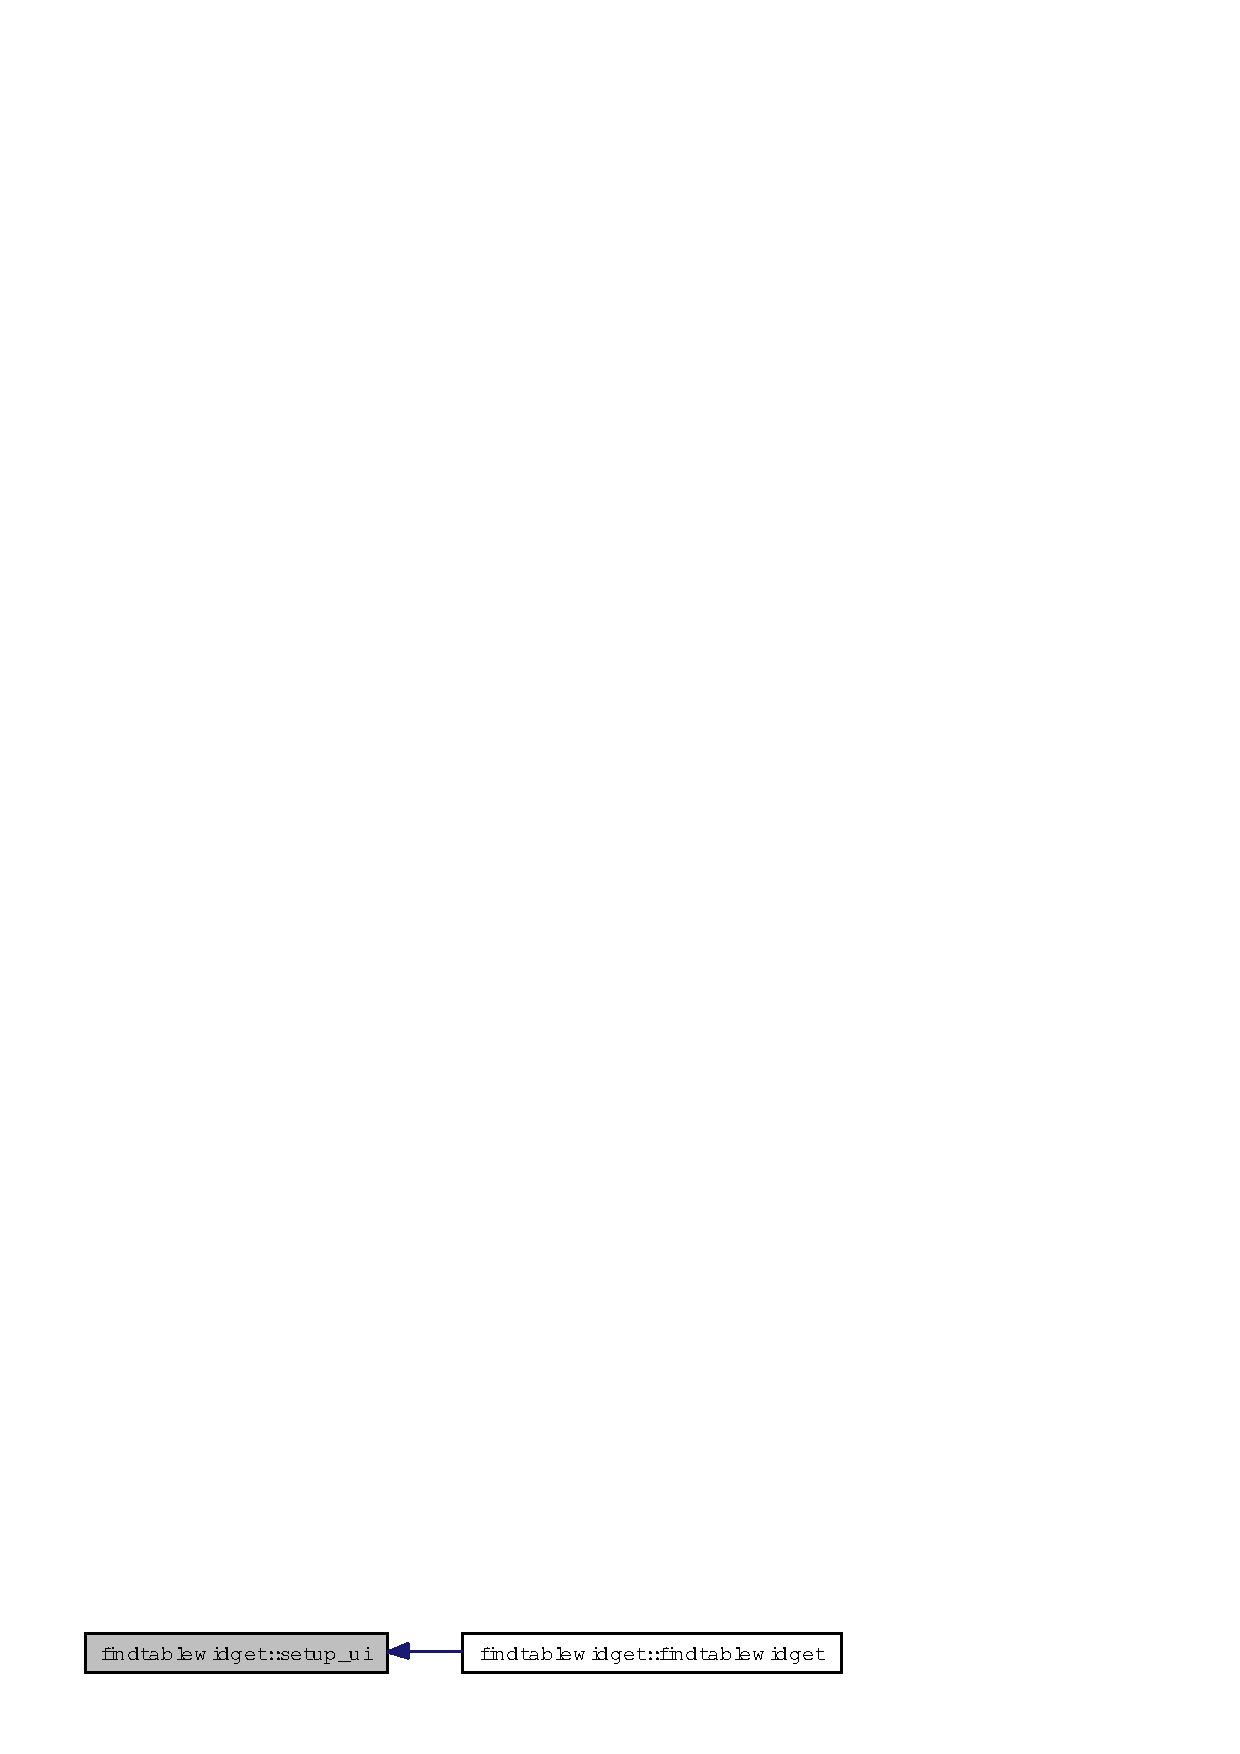
\includegraphics[width=204pt]{classfindtablewidget_a9a60fc112c853da5d244d2ef826ae80_icgraph}
\end{center}
\end{figure}
\index{findtablewidget@{findtablewidget}!setup_signals@{setup\_\-signals}}
\index{setup_signals@{setup\_\-signals}!findtablewidget@{findtablewidget}}
\subsubsection{\setlength{\rightskip}{0pt plus 5cm}void findtablewidget::setup\_\-signals (void)\hspace{0.3cm}{\tt  [private]}}\label{classfindtablewidget_e2b71d3917571b2d4558ebaa1fd382b9}




Definition at line 46 of file findtablewidget.cpp.

References findtableview, and select\_\-cell().

Referenced by findtablewidget().

Here is the caller graph for this function:\begin{figure}[H]
\begin{center}
\leavevmode
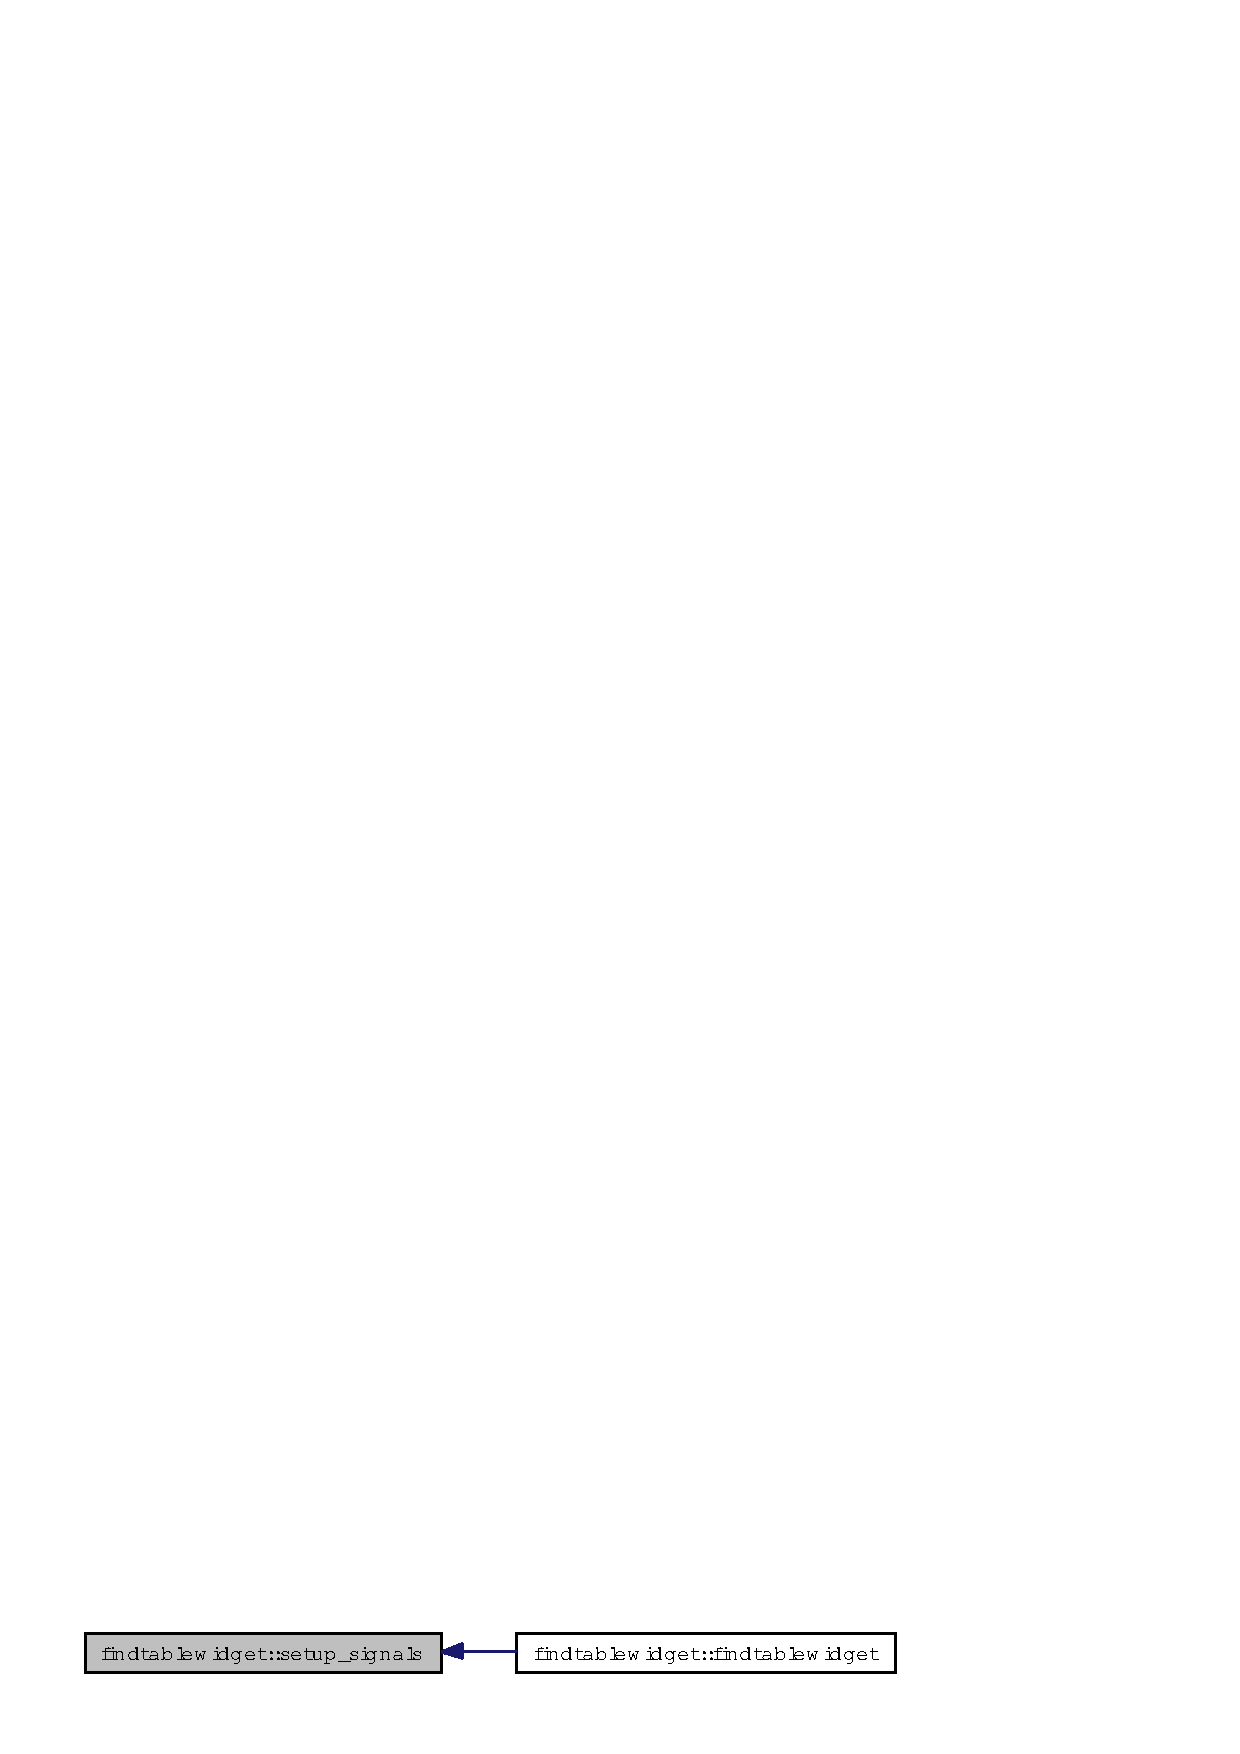
\includegraphics[width=217pt]{classfindtablewidget_e2b71d3917571b2d4558ebaa1fd382b9_icgraph}
\end{center}
\end{figure}
\index{findtablewidget@{findtablewidget}!assembly@{assembly}}
\index{assembly@{assembly}!findtablewidget@{findtablewidget}}
\subsubsection{\setlength{\rightskip}{0pt plus 5cm}void findtablewidget::assembly (void)\hspace{0.3cm}{\tt  [private]}}\label{classfindtablewidget_ce0d13010998778d2d9b18a76a66442d}




Definition at line 54 of file findtablewidget.cpp.

References findtableview.

Referenced by findtablewidget().

Here is the caller graph for this function:\begin{figure}[H]
\begin{center}
\leavevmode
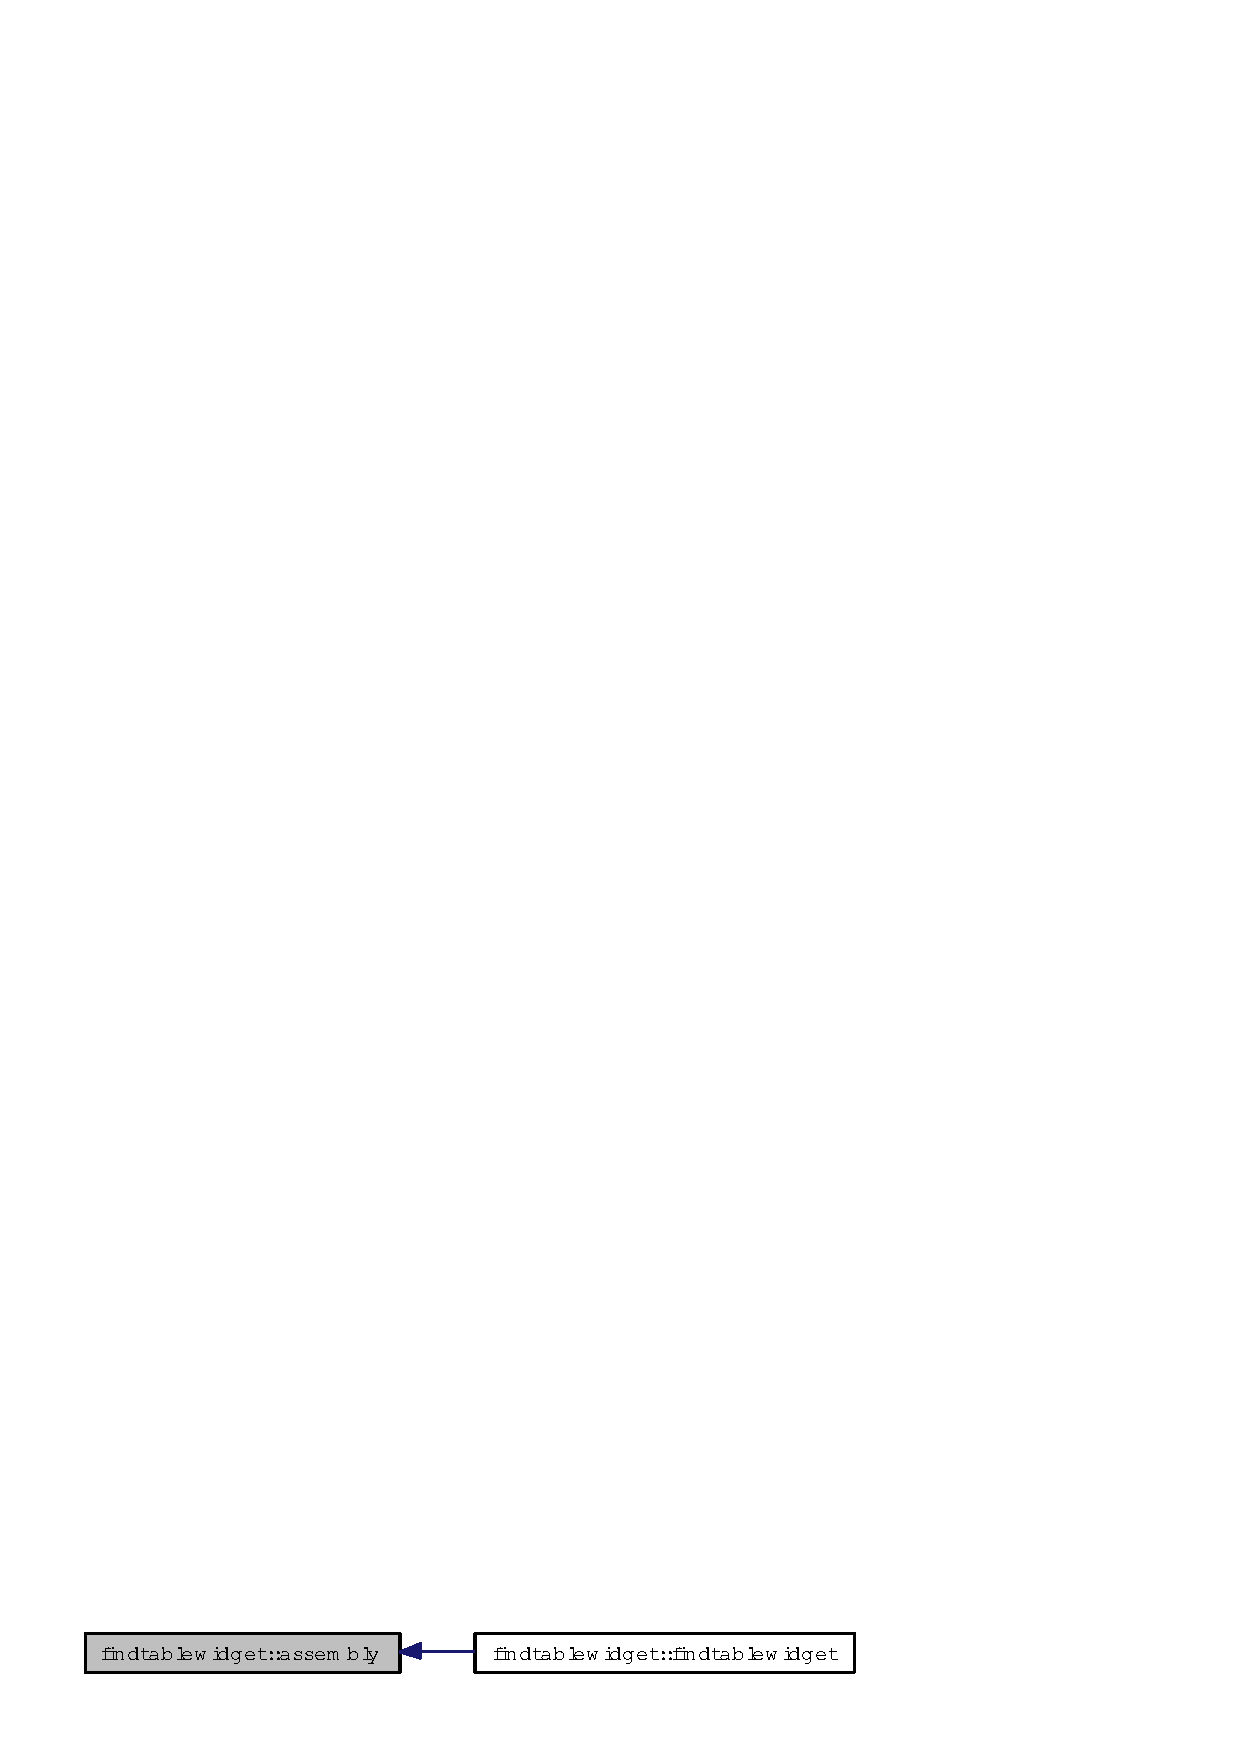
\includegraphics[width=207pt]{classfindtablewidget_ce0d13010998778d2d9b18a76a66442d_icgraph}
\end{center}
\end{figure}
\index{findtablewidget@{findtablewidget}!eventFilter@{eventFilter}}
\index{eventFilter@{eventFilter}!findtablewidget@{findtablewidget}}
\subsubsection{\setlength{\rightskip}{0pt plus 5cm}bool findtablewidget::event\-Filter (QObject $\ast$ {\em o}, QEvent $\ast$ {\em e})\hspace{0.3cm}{\tt  [private]}}\label{classfindtablewidget_37e8a0db7b8e6c0f6a48fcffdafc343c}




Definition at line 123 of file findtablewidget.cpp.

References findtableview.

\subsection{Member Data Documentation}
\index{findtablewidget@{findtablewidget}!findtableview@{findtableview}}
\index{findtableview@{findtableview}!findtablewidget@{findtablewidget}}
\subsubsection{\setlength{\rightskip}{0pt plus 5cm}QTable\-Widget$\ast$ {\bf findtablewidget::findtableview}\hspace{0.3cm}{\tt  [private]}}\label{classfindtablewidget_00c9dfe708d23bd0b80a476f40ab0cc3}




Definition at line 26 of file findtablewidget.h.

Referenced by add\_\-row(), assembly(), clear\_\-all(), event\-Filter(), select\_\-cell(), setup\_\-signals(), setup\_\-ui(), and update\_\-columns\_\-width().

The documentation for this class was generated from the following files:\begin{CompactItemize}
\item 
{\bf findtablewidget.h}\item 
{\bf findtablewidget.cpp}\end{CompactItemize}
